\documentclass[aspectratio=169,10pt]{ctexbeamer}

\usepackage{graphicx}
\usepackage{booktabs}
\usepackage{tikz}
\usetikzlibrary{arrows.meta,positioning,calc}

\definecolor{Navy}{HTML}{102A43}
\definecolor{Blue}{HTML}{1677A8}
\definecolor{Cyan}{HTML}{23A6B5}
\definecolor{Gray}{HTML}{5F6F7E}
\definecolor{Light}{HTML}{F2F6F8}
\definecolor{Line}{HTML}{D5E0E6}
\definecolor{Orange}{HTML}{D97706}

\usetheme{default}
\setbeamertemplate{navigation symbols}{}
\setbeamercolor{normal text}{fg=Navy,bg=white}
\setbeamercolor{structure}{fg=Blue}
\setbeamercolor{frametitle}{fg=Navy,bg=white}
\setbeamerfont{frametitle}{size=\Large,series=\bfseries}
\setbeamerfont{title}{size=\fontsize{21}{27},series=\bfseries}
\setbeamerfont{subtitle}{size=\large}
\setbeamertemplate{itemize item}{\color{Cyan}\raise0.15ex\hbox{\scriptsize$\blacktriangleright$}}
\setbeamertemplate{itemize subitem}{\color{Blue}\raise0.15ex\hbox{\tiny$\bullet$}}
\setbeamertemplate{blocks}[rounded][shadow=false]
\setbeamercolor{block title}{fg=white,bg=Blue}
\setbeamercolor{block body}{fg=Navy,bg=Light}

\setbeamertemplate{frametitle}{%
  \vspace{0.35em}\insertframetitle\par
  \vspace{-0.4em}\color{Cyan}\rule{1.0cm}{1.4pt}%
}
\setbeamertemplate{footline}{%
  \leavevmode\hbox{%
    \begin{beamercolorbox}[wd=.84\paperwidth,ht=2.7ex,dp=1.1ex,leftskip=.55cm]{author in head/foot}
      \color{Gray}\scriptsize 吃福是亏 · 基于 HarmonyOS 的透明泡泡实时折射与色散渲染系统
    \end{beamercolorbox}%
    \begin{beamercolorbox}[wd=.16\paperwidth,ht=2.7ex,dp=1.1ex,rightskip=.55cm plus1fil]{date in head/foot}
      \color{Blue}\scriptsize\hfill\insertframenumber\,/\,\inserttotalframenumber
    \end{beamercolorbox}%
  }%
}

\tikzset{
  flow/.style={rounded corners=3pt,draw=Blue,fill=Blue!6,minimum width=2.18cm,
    minimum height=.82cm,align=center,font=\scriptsize\bfseries},
  smallflow/.style={rounded corners=3pt,draw=Cyan,fill=Cyan!6,minimum width=1.75cm,
    minimum height=.72cm,align=center,font=\scriptsize},
  arrow/.style={-{Latex[length=2.1mm]},draw=Gray,line width=.9pt}
}

\graphicspath{{../documents/}{../homepage/}{../}}

\title{基于 HarmonyOS 的\\透明泡泡实时折射与色散\\渲染系统}
\subtitle{CCF CAD/CG 2026 高质量实时渲染技术挑战赛}
\author{队伍：吃福是亏}
\date{}

\begin{document}

{\setbeamertemplate{footline}{}
\begin{frame}[plain]
  \vfill
  \begin{center}
  \begin{minipage}{0.72\textwidth}
    \centering
    {\color{Cyan}\rule{1.15cm}{2pt}}\par
    \vspace{0.55cm}
    {\usebeamerfont{title}\color{Navy}\inserttitle\par}
    \vspace{0.4cm}
    {\usebeamerfont{subtitle}\color{Blue}\insertsubtitle\par}
    \vspace{0.85cm}
    {\small
    \begin{tabular}{@{}ll@{}}
      \textcolor{Gray}{队伍名称} & \textbf{吃福是亏}\\[0.12cm]
      \textcolor{Gray}{队伍成员} & 杨弘宇、常毅寒、杨硕、高凡、赵艺博\\[0.12cm]
      \textcolor{Gray}{指导老师} & 蔡有城\\
    \end{tabular}}
    \vspace{0.45cm}

    {\color{Gray}\scriptsize 中国科学技术大学}
  \end{minipage}
  \end{center}
  \vfill
\end{frame}}

\begin{frame}{项目目标与最终成果}
  \begin{columns}[T,onlytextwidth]
    \column{0.56\textwidth}
      \begin{block}{赛题目标}
        在 HarmonyOS 设备上实现透明物体的实时折射、色散、动态模拟与触控交互，并形成完整可运行的演示系统。
      \end{block}
      \vspace{0.2cm}
      \begin{itemize}\setlength\itemsep{0.48em}
        \item 以肥皂泡为对象，统一表现透明折射、薄膜虹彩和动态表面
        \item 采用多阶段 FBO，在光栅化管线中近似双界面折射
        \item 实现 Kim2012 与 Belcour Airy 两种虹彩模式
        \item 接入 DBSTT 风格形变、触摸波纹和多泡泡漂移
        \item 完成 ArkTS 界面、Native 渲染和真机运行链路
      \end{itemize}
    \column{0.40\textwidth}
      \centering
      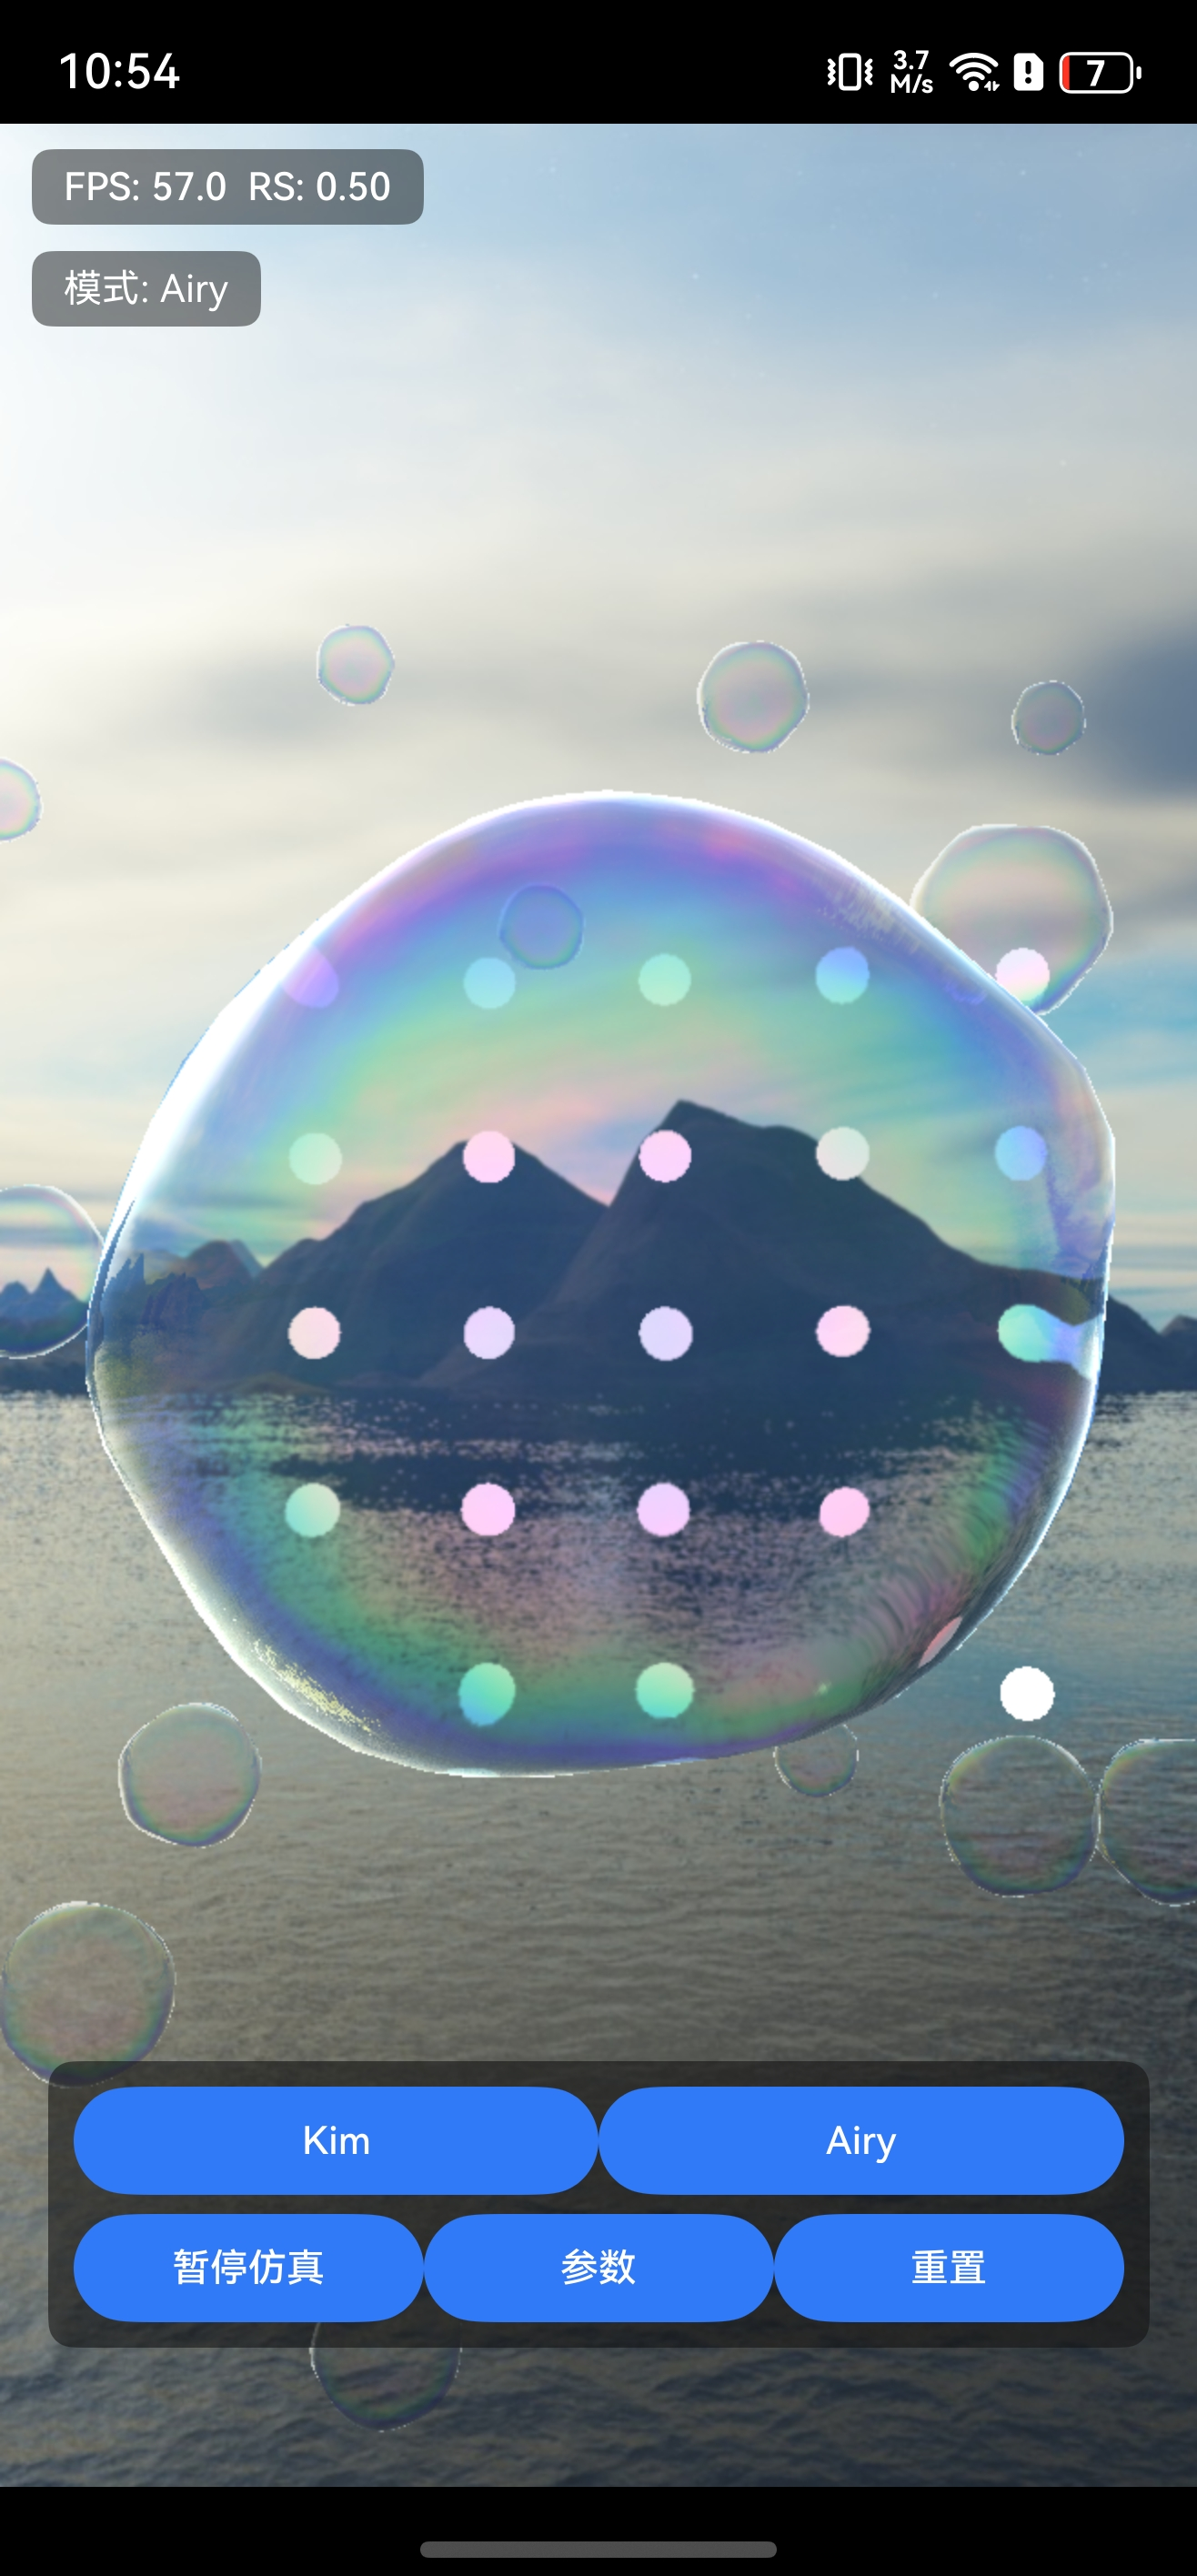
\includegraphics[height=5.85cm,trim=0 130 0 160,clip]{bubble_harm1.jpg}
      \par\vspace{0.1cm}
      \scriptsize\color{Gray}HarmonyOS 真机运行效果
  \end{columns}
\end{frame}

\begin{frame}{系统架构：ArkTS 页面与 Native 渲染协同}
  \centering
  \vspace{0.2cm}
  \begin{tikzpicture}[node distance=.45cm]
    \node[flow] (ark) {ArkTS 页面层\\按钮、滑杆、触控};
    \node[flow,right=of ark] (xc) {XComponent\\Surface 渲染画布};
    \node[flow,right=of xc] (napi) {NAPI / libentry.so\\跨语言参数接口};
    \node[flow,right=of napi] (cpp) {C++ Native\\渲染与物理模拟};
    \draw[arrow] (ark)--(xc); \draw[arrow] (xc)--(napi); \draw[arrow] (napi)--(cpp);

    \node[smallflow,below=.72cm of ark] (touch) {触控与 UI 状态};
    \node[smallflow,below=.72cm of xc] (egl) {EGL Context};
    \node[smallflow,below=.72cm of napi] (gl) {OpenGL ES 3.0};
    \node[smallflow,below=.72cm of cpp] (res) {FBO / Shader / DBSTT};
    \draw[arrow] (touch)--(egl); \draw[arrow] (egl)--(gl); \draw[arrow] (gl)--(res);
  \end{tikzpicture}
  \vspace{0.65cm}
  \begin{columns}[T,onlytextwidth]
    \column{0.47\textwidth}
      \textbf{页面与交互}
      \begin{itemize}\setlength\itemsep{0.35em}
        \item XComponent 承载原生画面
        \item 单指、双指和参数面板输入
        \item FPS、当前模式与仿真状态显示
      \end{itemize}
    \column{0.47\textwidth}
      \textbf{Native 核心}
      \begin{itemize}\setlength\itemsep{0.35em}
        \item EGL 创建 OpenGL ES 3.0 上下文
        \item rawfile 加载天空盒与纹理资源
        \item 多 Pass 渲染、动态网格与资源管理
      \end{itemize}
  \end{columns}
\end{frame}

\begin{frame}{五阶段 FBO：移动端双界面折射近似}
  \centering
  \begin{tikzpicture}[node distance=.28cm]
    \node[flow] (p1) {背景阶段\\backgroundFBO};
    \node[flow,right=of p1] (p2) {后景阶段\\sceneBehindFBO};
    \node[flow,right=of p2] (p3) {背面阶段\\backFaceFBO};
    \node[flow,right=of p3] (p4) {主场景阶段\\mainSceneFBO};
    \node[flow,right=of p4] (p5) {最终合成\\finalSceneFBO};
    \draw[arrow] (p1)--(p2); \draw[arrow] (p2)--(p3);
    \draw[arrow] (p3)--(p4); \draw[arrow] (p4)--(p5);
  \end{tikzpicture}
  \vspace{0.65cm}
  \begin{columns}[T,onlytextwidth]
    \column{0.51\textwidth}
      \textbf{设计思想}
      \begin{itemize}\setlength\itemsep{0.48em}
        \item 背景先成为可被折射采样的纹理
        \item 前、背表面分两次计算折射偏移
        \item 主泡泡结果再作为展示泡泡的采样输入
        \item 透明对象按相机距离排序并进行 Alpha 合成
      \end{itemize}
    \column{0.45\textwidth}
      \begin{block}{性能取舍}
        内部 FBO 使用屏幕宽高的 \(0.5\) 倍，再由全屏四边形放大；通过坐标修正保证窗口像素与 FBO 像素一致。
      \end{block}
      \vspace{0.2cm}
      {\scriptsize\color{Gray}
      优点：完全运行在 GPU 光栅化管线中。\\
      局限：只能折射已经出现在屏幕纹理中的内容。}
  \end{columns}
\end{frame}

\begin{frame}{屏幕空间折射：中心清透，轮廓增强}
  \begin{columns}[T,onlytextwidth]
    \column{0.55\textwidth}
      \begin{block}{折射方向}
        \[
          \eta=\frac{n_{\mathrm{air}}}{n_{\mathrm{film}}}=\frac{1.0}{1.33},
          \qquad
          \mathbf{T}=\operatorname{refract}(\mathbf{V},\mathbf{N},\eta)
        \]
      \end{block}
      \begin{itemize}\setlength\itemsep{0.46em}
        \item 使用 \(\mathbf{T}_{xy}\) 形成背景纹理的屏幕空间采样偏移
        \item 用 \(e=1-|\mathbf{V}\cdot\mathbf{N}|\) 描述轮廓程度
        \item 背面 Pass 使用较小系数，避免双界面叠加后过度扭曲
        \item 最大偏移限制为泡泡屏幕半径的一定比例，抑制跳变
      \end{itemize}
    \column{0.41\textwidth}
      \centering
      \begin{tikzpicture}[scale=.72]
        \shade[ball color=Cyan!25,opacity=.62] (0,0) circle (2.15);
        \draw[Blue,line width=1.2pt] (0,0) circle (2.15);
        \draw[-{Latex},Gray,line width=1.1pt] (-3.0,1.25)--(-1.7,.85);
        \draw[-{Latex},Orange,line width=1.3pt] (-1.7,.85)--(.15,-.05);
        \draw[-{Latex},Blue,line width=1.3pt] (.15,-.05)--(2.8,-.72);
        \draw[dashed,Gray] (-1.7,.85)--(-.85,2.5);
        \node[font=\scriptsize,text=Gray] at (-2.55,1.55) {入射};
        \node[font=\scriptsize,text=Orange] at (-.75,.18) {背面折射};
        \node[font=\scriptsize,text=Blue] at (2.0,-.25) {正面折射};
      \end{tikzpicture}
      \par\vspace{0.2cm}
      \scriptsize\color{Gray}两个屏幕空间界面近似薄壳传播
  \end{columns}
\end{frame}

\begin{frame}{薄膜虹彩：两种实时实现路径}
  \small
  \[
    \phi_\lambda=\frac{4\pi n d\cos\theta_t}{\lambda}
  \]
  \vspace{-0.1cm}
  \begin{tabular}{@{}p{2.25cm}p{3.55cm}p{3.35cm}p{3.2cm}@{}}
    \toprule
    \textbf{模式} & \textbf{计算方式} & \textbf{特点} & \textbf{用途与局限}\\
    \midrule
    \textcolor{Blue}{\textbf{Kim2012}} &
    Shader 实时计算 615/535/465 nm 三个代表波长 &
    公式直观，便于展示相位差与 Fresnel 系数 &
    光谱连续性有限，颜色可能偏强\\
    \addlinespace
    \textcolor{Orange}{\textbf{Belcour Airy}} &
    以 7 个波长近似 Airy 多次内反射 &
    颜色过渡与环境反射更自然 &
    当前默认模式；属于项目级简化\\
    \bottomrule
  \end{tabular}
\end{frame}

\begin{frame}{动态膜厚与最终颜色合成}
  \begin{columns}[T,onlytextwidth]
    \column{0.55\textwidth}
      \textbf{程序化膜厚场}
      \[
        d=d_0+A_{\mathrm{var}}P(\mathbf{n},t)
          +190M_{\mathrm{touch}}+95Q_{\mathrm{ripple}}
      \]
      \begin{itemize}\setlength\itemsep{0.44em}
        \item \(P(\mathbf{n},t)\)：多层 Simplex noise、缓慢流动和重力排液趋势
        \item 以世界法线方向作为噪声输入，避免球体 UV 接缝
        \item 触摸中心和环状波纹直接改变局部膜厚
      \end{itemize}
    \column{0.41\textwidth}
      \textbf{颜色组成}
      \begin{enumerate}\setlength\itemsep{0.48em}
        \item 折射采样得到的透射背景
        \item 当前光学模式计算的薄膜反射率
        \item Cubemap 环境反射与少量高光
      \end{enumerate}
      \vspace{0.25cm}
      \begin{block}{Fresnel 边缘项}
        \[
          F=(1-|\mathbf{V}\cdot\mathbf{N}|)^p
        \]
        中心保持透明，轮廓处增强反射与虹彩。
      \end{block}
  \end{columns}
\end{frame}

\begin{frame}{DBSTT：用涡流片驱动主泡泡表面形变}
  \begin{columns}[T,onlytextwidth]
    \column{0.56\textwidth}
      \textbf{核心思想}
      \begin{itemize}\setlength\itemsep{0.42em}
        \item 仅离散泡泡表面，不求解完整体积 Navier--Stokes
        \item 以逐顶点环量 \(\Gamma\) 描述涡流片状态
        \item 由表面梯度得到涡流片强度，再通过 Biot--Savart 恢复速度
      \end{itemize}
      \[
        \boldsymbol{\gamma}=\mathbf{n}\times\nabla_f\Gamma,
        \qquad
        \mathbf{u}(\mathbf{x})=\frac{1}{4\pi}\int_S
        \boldsymbol{\gamma}(\mathbf{x}')\times
        \frac{\mathbf{x}-\mathbf{x}'}{|\mathbf{x}-\mathbf{x}'|^3}\,df'
      \]
      \begin{block}{本项目实现范围}
        简化为单个闭合泡泡的表面动态；不包含非流形拓扑变化、泡沫区域标记和 Plateau 边界。
      \end{block}
    \column{0.40\textwidth}
      \centering
      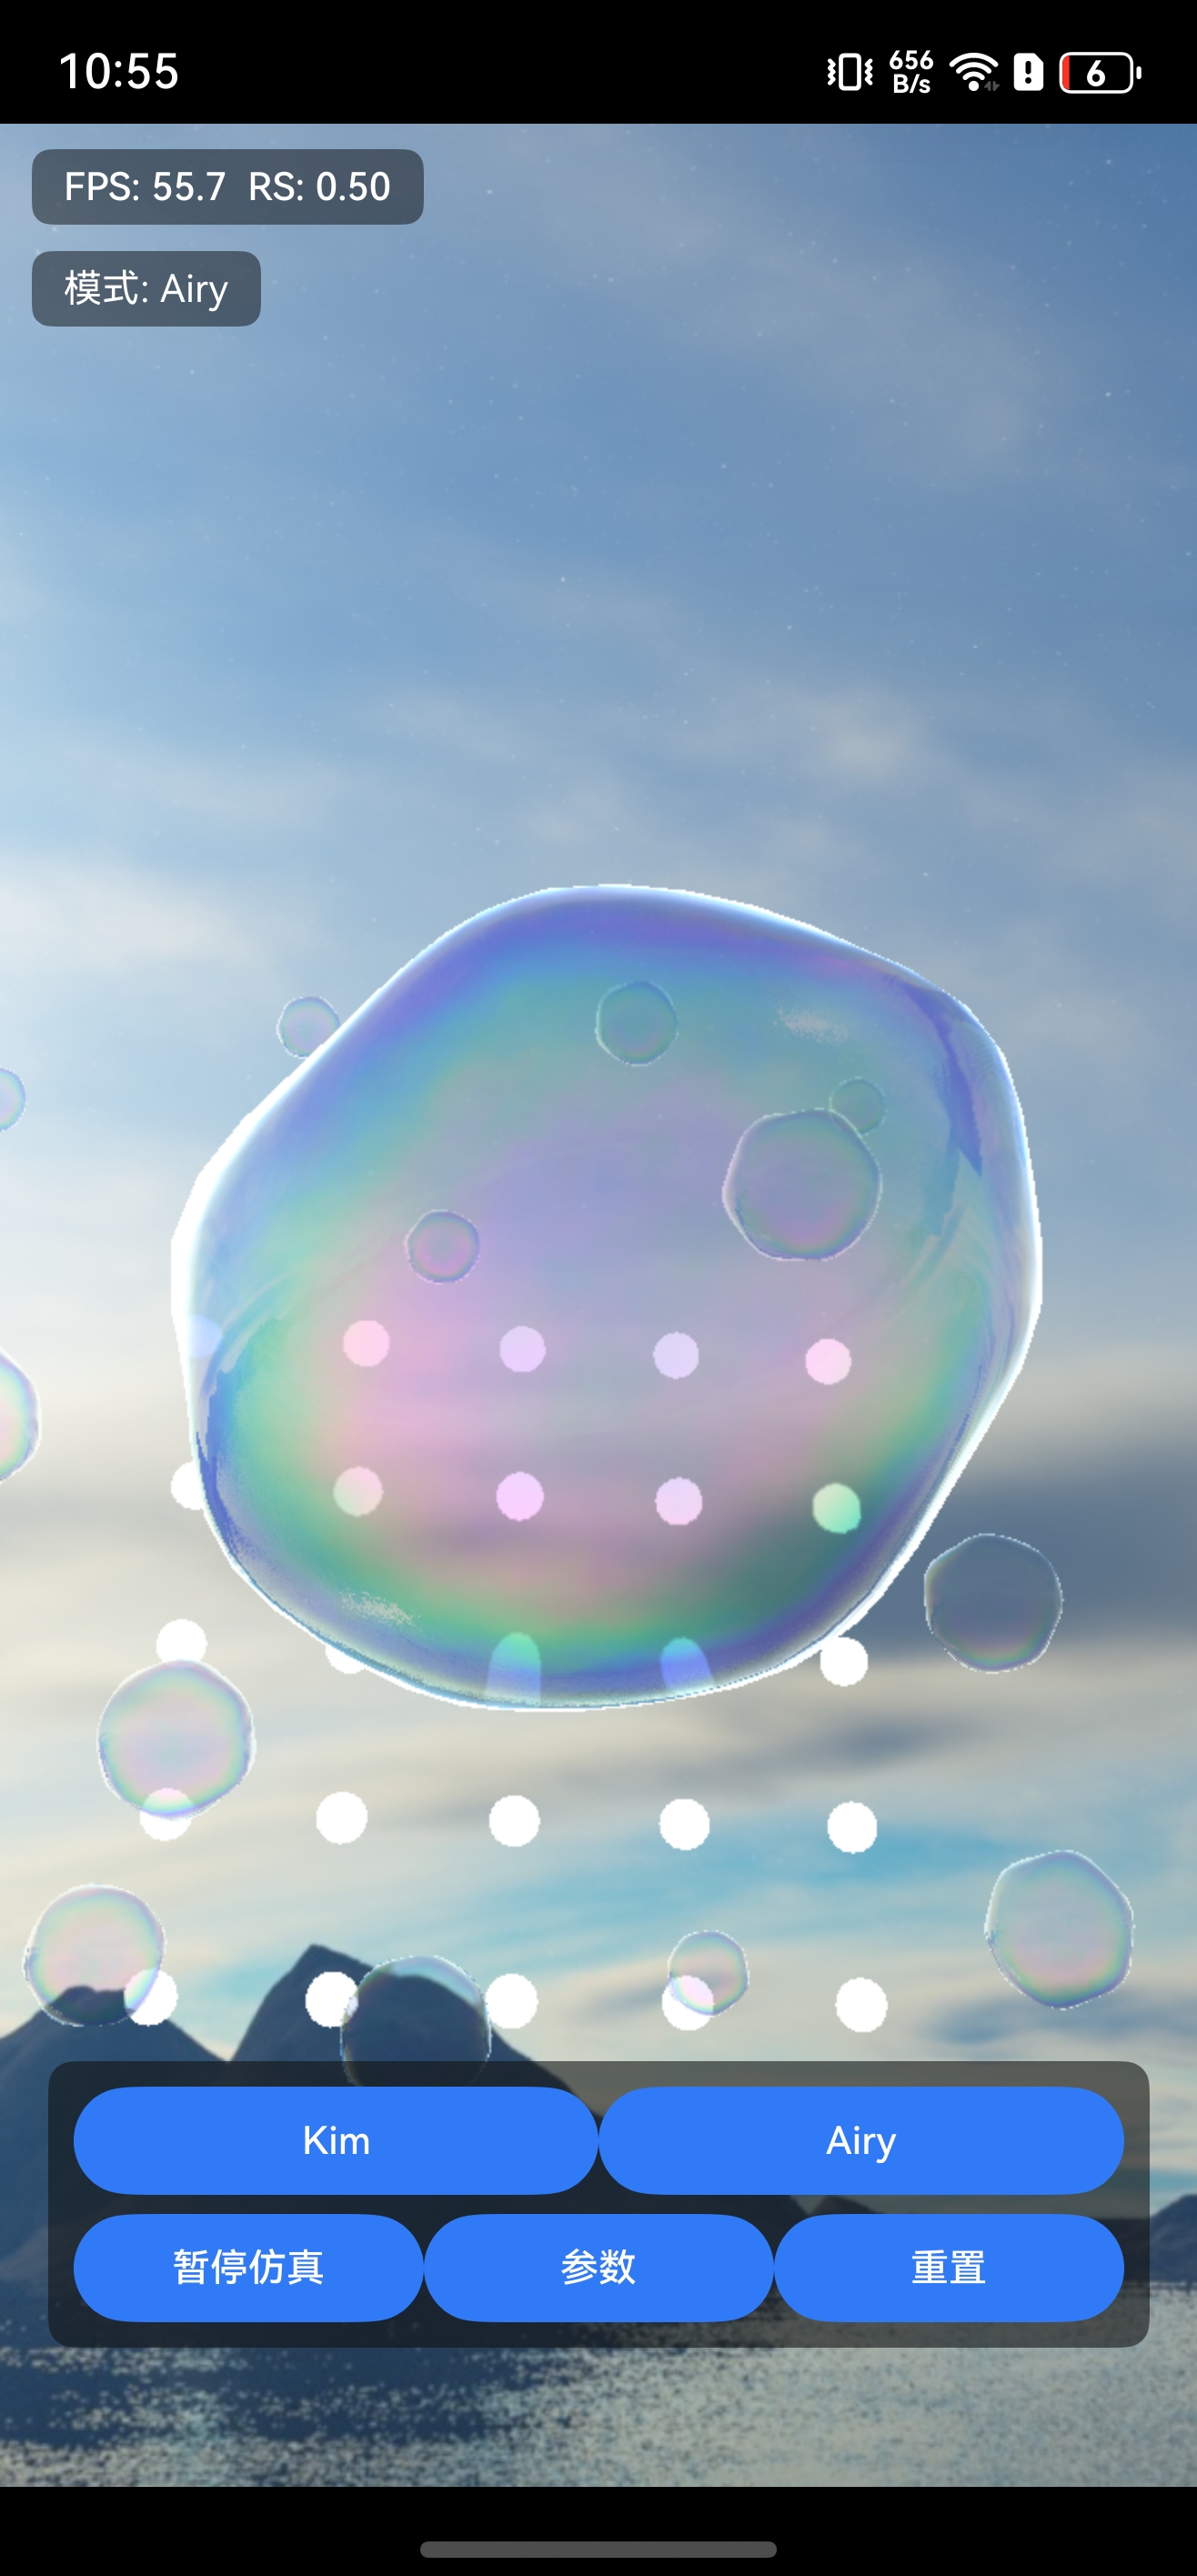
\includegraphics[height=5.75cm,trim=0 180 0 180,clip]{bubble_ham2.jpg}
      \par\vspace{0.1cm}
      \scriptsize\color{Gray}真机上的非球形主泡泡轮廓
  \end{columns}
\end{frame}

\begin{frame}{物理模拟与移动端渲染的集成}
  \begin{columns}[T,onlytextwidth]
    \column{0.53\textwidth}
      \begin{tikzpicture}[node distance=.24cm]
        \node[smallflow] (a) {几何量与曲率};
        \node[smallflow,below=of a] (b) {表面张力积分};
        \node[smallflow,below=of b] (c) {环量扩散};
        \node[smallflow,below=of c] (d) {Biot--Savart 速度};
        \node[smallflow,below=of d] (e) {位置推进与法线更新};
        \draw[arrow] (a)--(b); \draw[arrow] (b)--(c);
        \draw[arrow] (c)--(d); \draw[arrow] (d)--(e);
        \node[right=.35cm of c,align=left,font=\scriptsize,text=Gray] {
          前向欧拉积分\\
          位移钳制：\(0.1\bar e\)\\
          质心归零抑制漂移};
      \end{tikzpicture}
    \column{0.43\textwidth}
      \textbf{针对移动端的降频策略}
      \begin{itemize}\setlength\itemsep{0.48em}
        \item icosphere 半径 \(R=1.5\)，初始拉伸扰动 16\%
        \item 每次实际更新只执行 1 个子步
        \item 时间步长 \(\Delta t=0.001\) 秒
        \item 每隔 6 个渲染帧推进一次 CPU 仿真
        \item 更新后上传顶点与法线到 VBO
      \end{itemize}
      \vspace{0.2cm}
      {\scriptsize\color{Gray}
      低频物理形变负责轮廓变化，Shader 连续扰动保证视觉运动不间断。}
  \end{columns}
\end{frame}

\begin{frame}{触摸交互：从手势到局部光学响应}
  \begin{columns}[T,onlytextwidth]
    \column{0.58\textwidth}
      \begin{tikzpicture}[node distance=.3cm,scale=.82,transform shape]
        \node[smallflow] (t1) {ArkTS TouchEvent};
        \node[smallflow,right=of t1] (t2) {XComponent 局部坐标};
        \node[smallflow,right=of t2] (t3) {NAPI};
        \node[smallflow,right=of t3] (t4) {Shader / Camera};
        \draw[arrow] (t1)--(t2); \draw[arrow] (t2)--(t3); \draw[arrow] (t3)--(t4);
      \end{tikzpicture}
      \vspace{0.45cm}
      \begin{itemize}\setlength\itemsep{0.46em}
        \item \textbf{单指拖动：}改变相机 yaw/pitch
        \item \textbf{双指缩放：}调整相机距离
        \item \textbf{点击或短按：}在主泡泡上建立局部高斯影响区域
        \item \textbf{轻微移动：}根据触摸速度增强衰减环状波纹
      \end{itemize}
      \[
        M_{\mathrm{touch}}=
        \exp\!\left(-\frac{\|\mathbf{x}-\mathbf{x}_t\|^2}{r^2}\right)S_{\mathrm{touch}}
      \]
      {\scriptsize\color{Gray}
      触摸同时改变折射偏移与膜厚场，因此局部背景扭曲和虹彩会同步响应。}
    \column{0.37\textwidth}
      \centering
      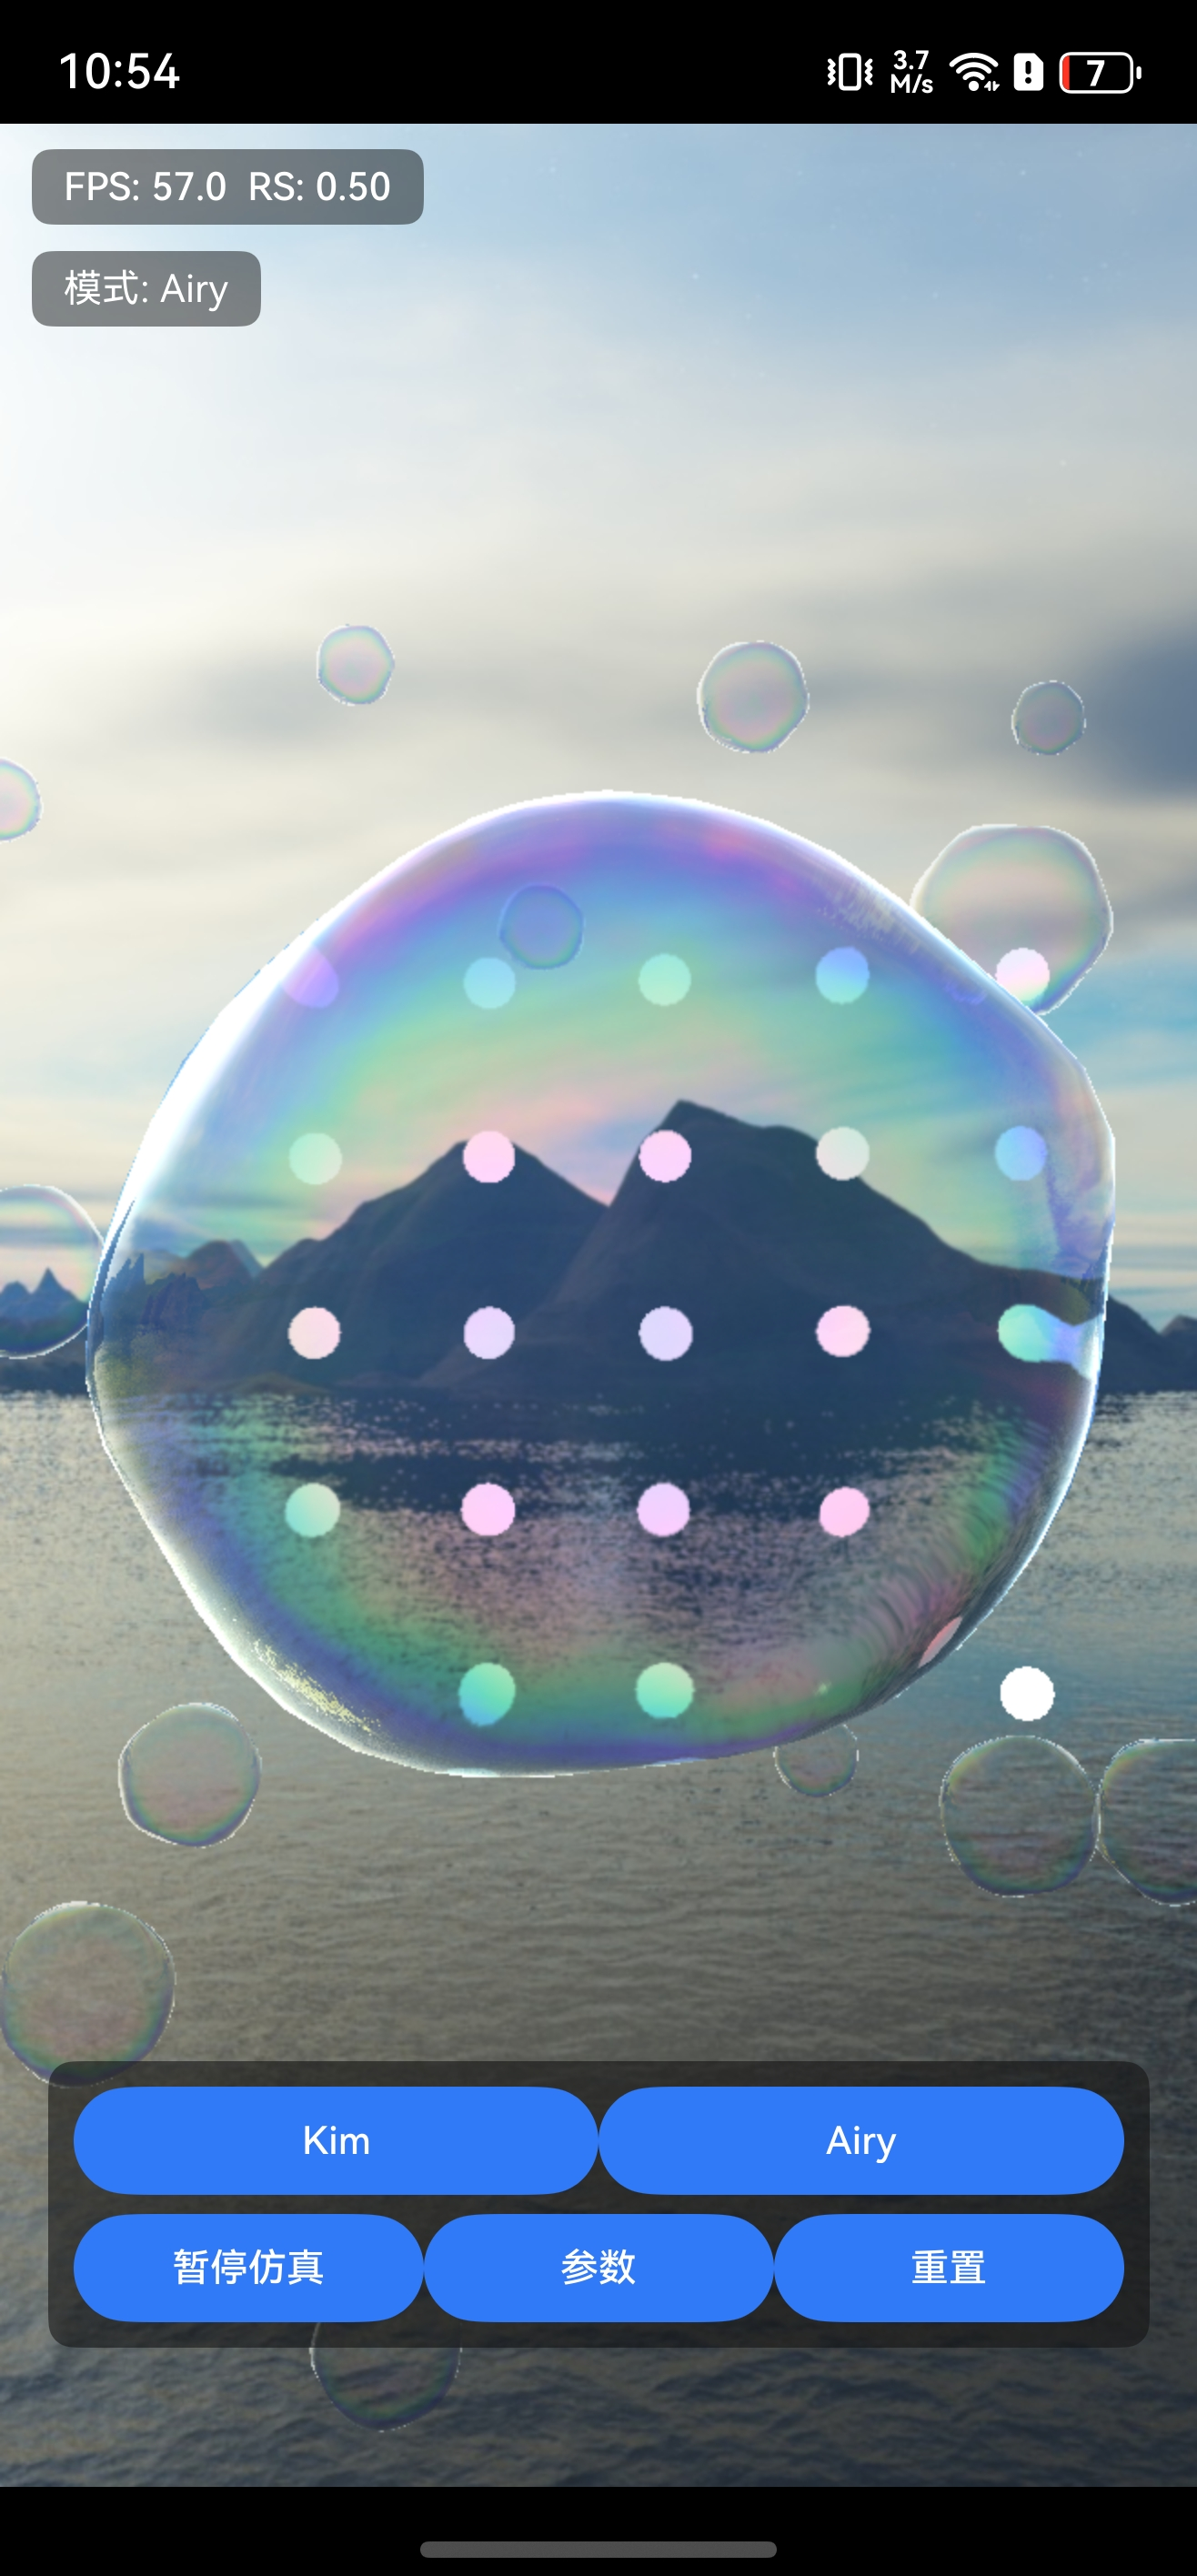
\includegraphics[height=5.9cm,trim=0 150 0 140,clip]{bubble_harm1.jpg}
  \end{columns}
\end{frame}

\begin{frame}{移动端界面：现场演示与参数控制}
  \begin{columns}[T,onlytextwidth]
    \column{0.39\textwidth}
      \centering
      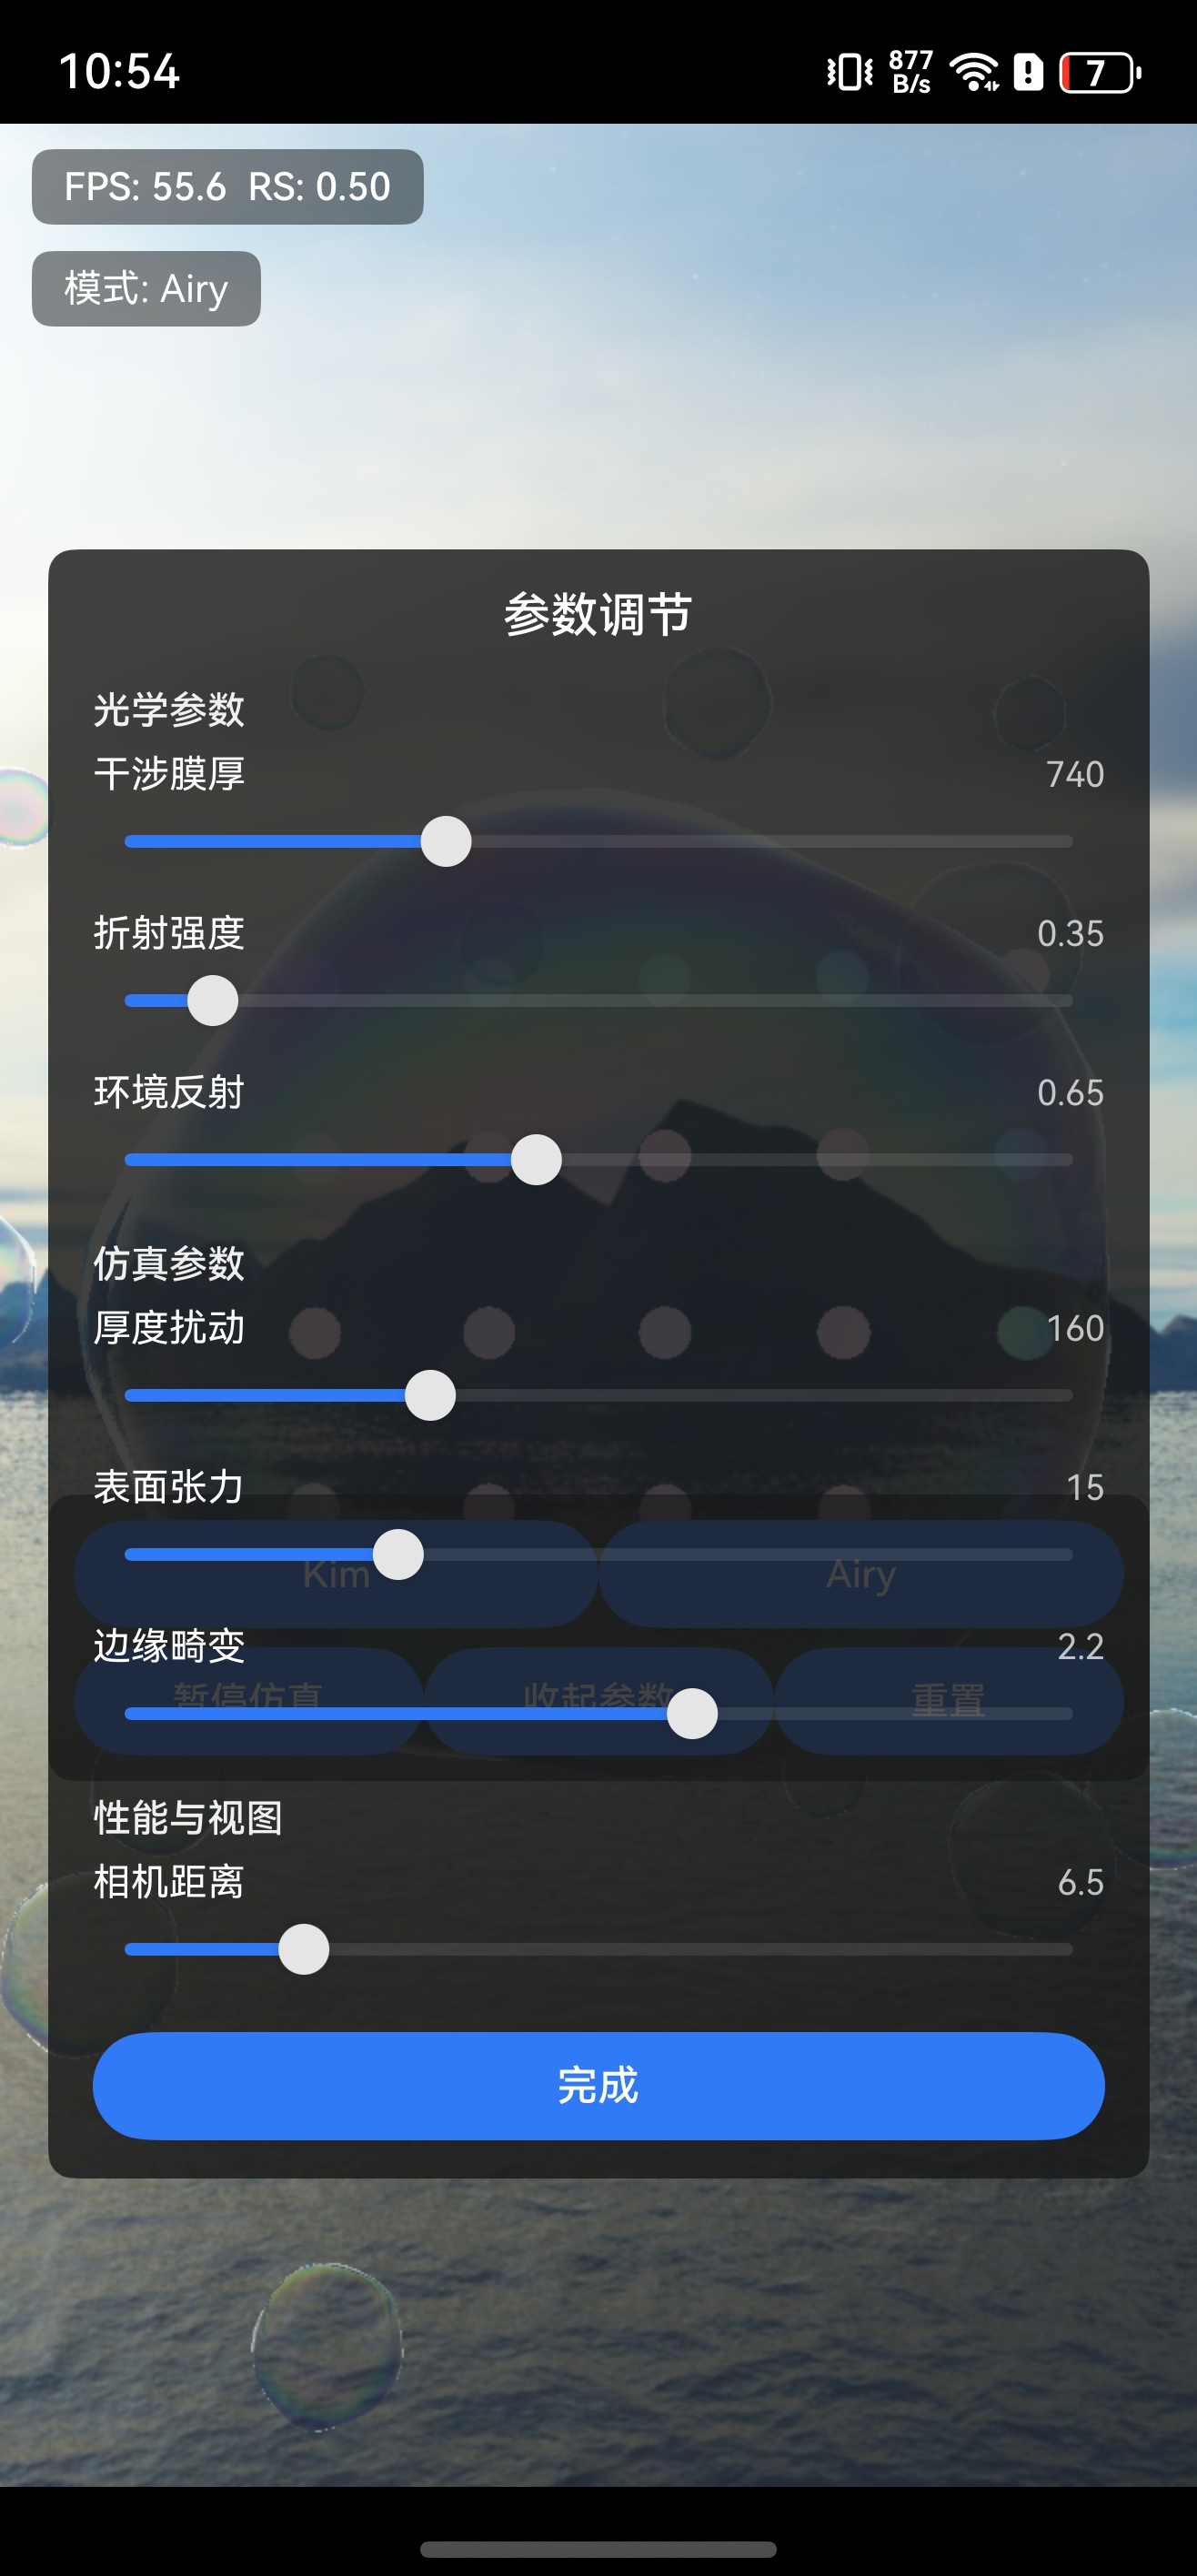
\includegraphics[height=6.1cm,trim=0 120 0 120,clip]{bubble_console.jpg}
    \column{0.57\textwidth}
      \textbf{界面开放的控制项}
      \begin{itemize}\setlength\itemsep{0.42em}
        \item \textbf{模式切换：}Kim / Airy，对比实时 RGB 与多波长 Airy
        \item \textbf{光学参数：}干涉膜厚、折射强度、环境反射
        \item \textbf{仿真参数：}厚度扰动、表面张力、边缘畸变
        \item \textbf{视图参数：}相机距离
        \item \textbf{状态控制：}暂停仿真、重置、FPS 与当前模式显示
      \end{itemize}
      \vspace{0.4cm}
      \begin{block}{参数链路}
        ArkTS 滑杆更新状态后，通过 NAPI 直接写入 Native 渲染参数，画面在下一帧即时反馈。
      \end{block}
  \end{columns}
\end{frame}

\begin{frame}{多泡泡展示与风吹漂移}
  \begin{columns}[T,onlytextwidth]
    \column{0.46\textwidth}
      \centering
      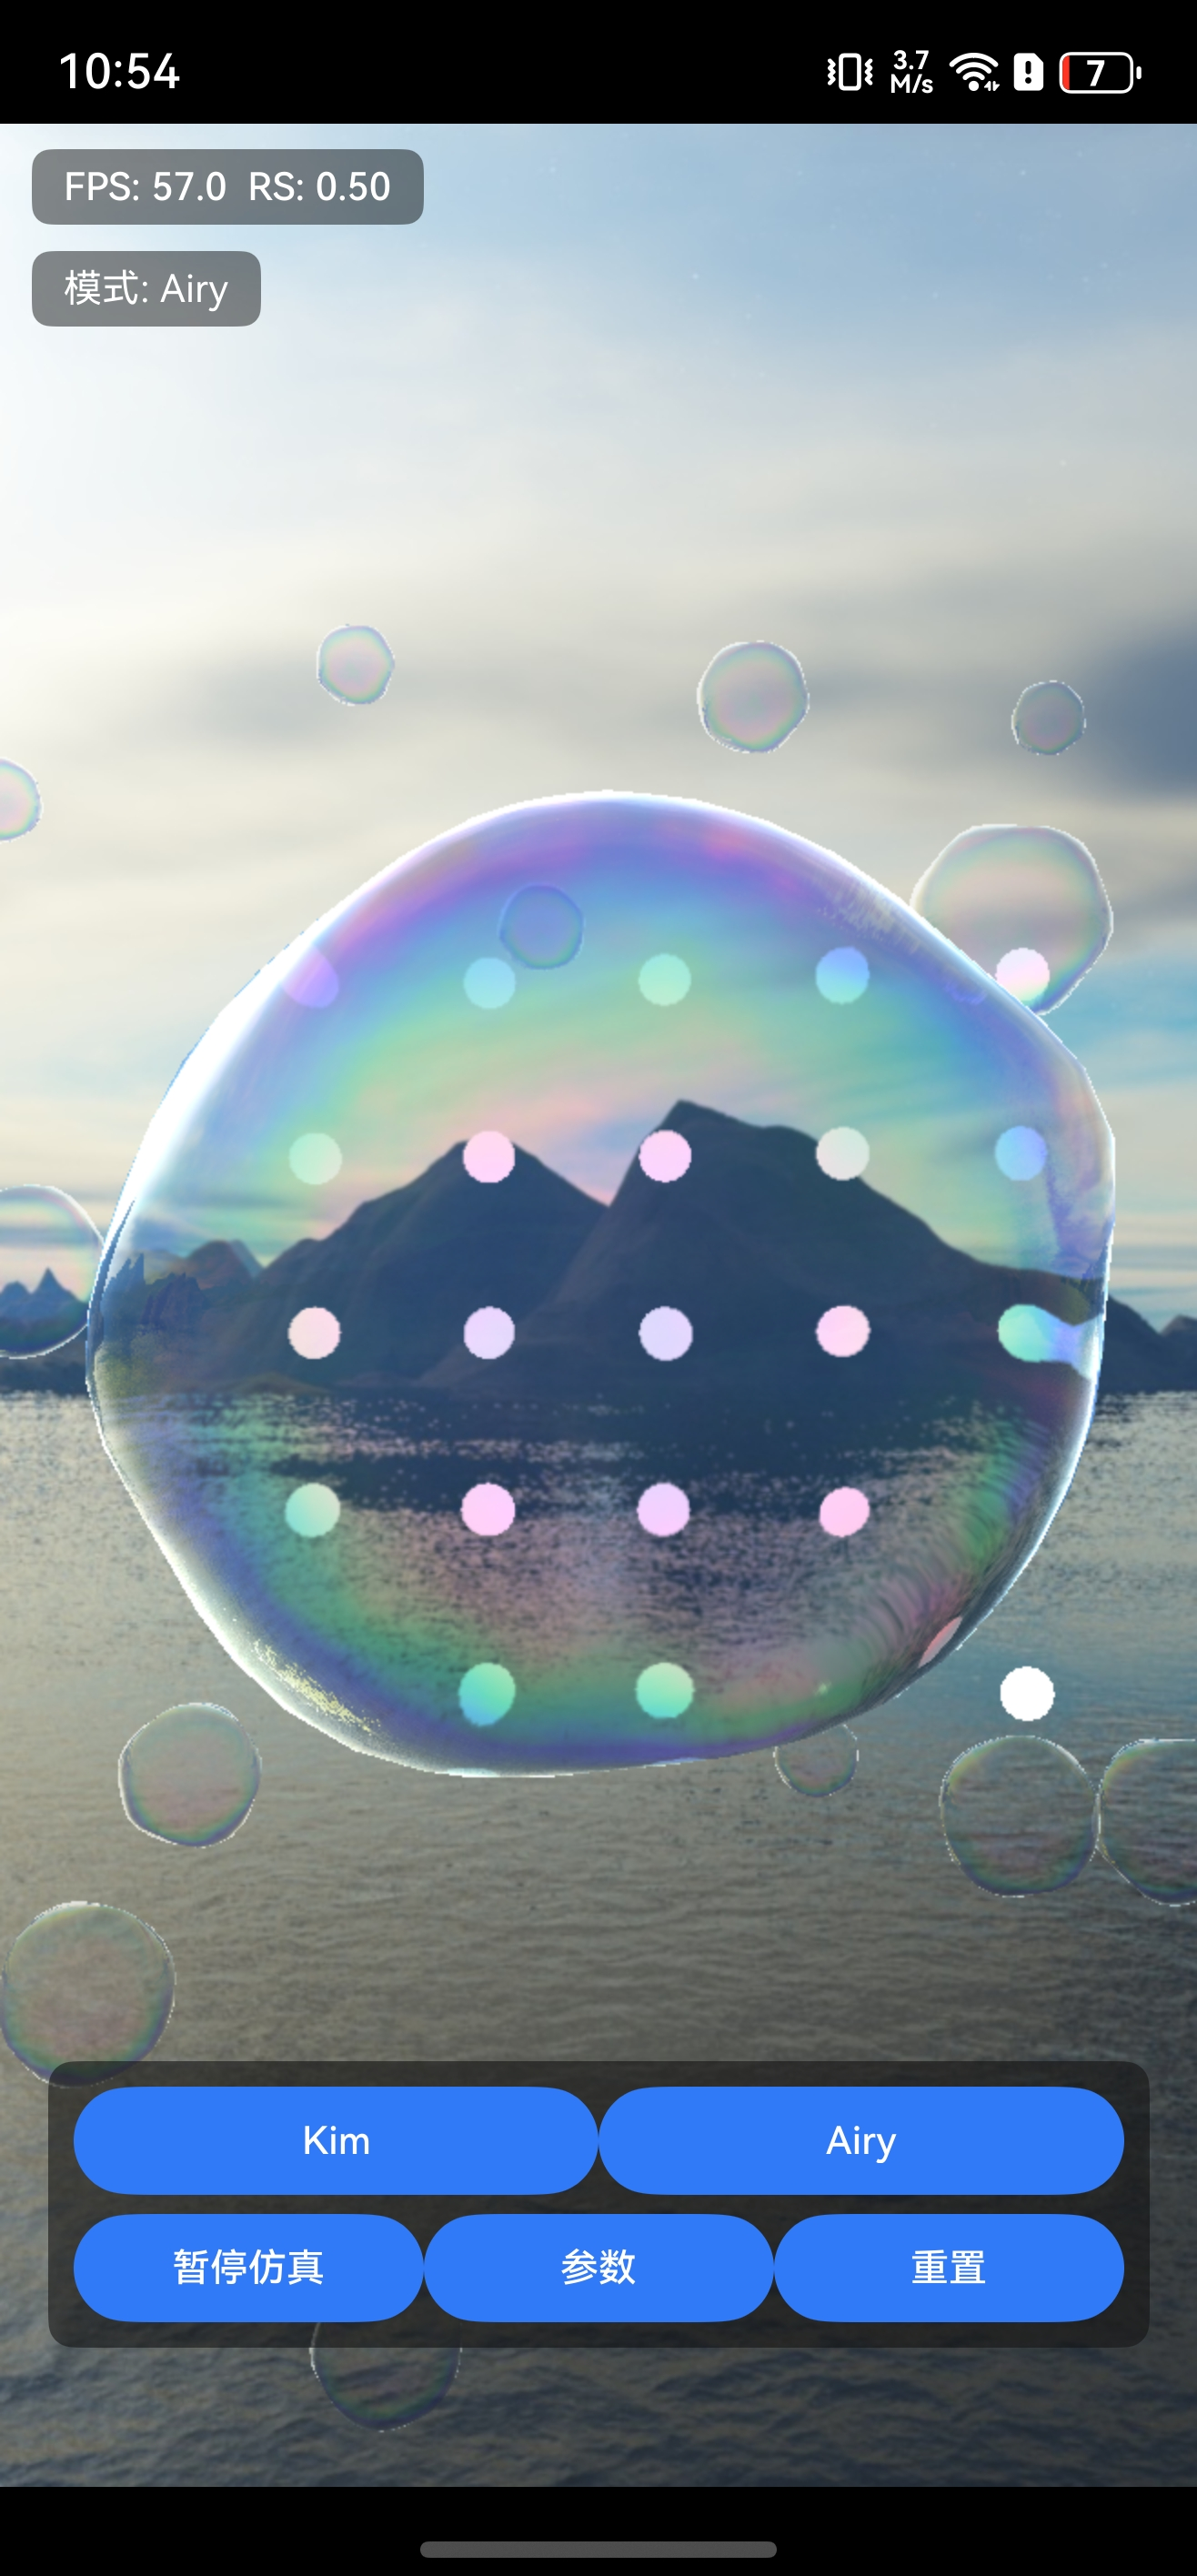
\includegraphics[height=5.85cm,trim=0 180 0 170,clip]{bubble_harm1.jpg}
    \column{0.50\textwidth}
      \textbf{场景组织}
      \begin{itemize}\setlength\itemsep{0.45em}
        \item 1 个 DBSTT 主泡泡与 16 个展示泡泡
        \item 展示泡泡共享折射/虹彩 Shader，不运行独立物理模拟
        \item 每个泡泡具有位置、半径、相位、风向振幅和速度
        \item 以正弦/余弦组合实现轻微漂移与 wobble
        \item 前后景混合排布，按相机距离从远到近排序
      \end{itemize}
      \vspace{0.2cm}
      \begin{block}{设计目的}
        在可控开销下丰富空间层次，同时避免为每个副泡泡复制昂贵的 CPU 表面模拟。
      \end{block}
  \end{columns}
\end{frame}

\begin{frame}{HarmonyOS 真机运行结果}
  \begin{columns}[T,onlytextwidth]
    \column{0.33\textwidth}
      \centering
      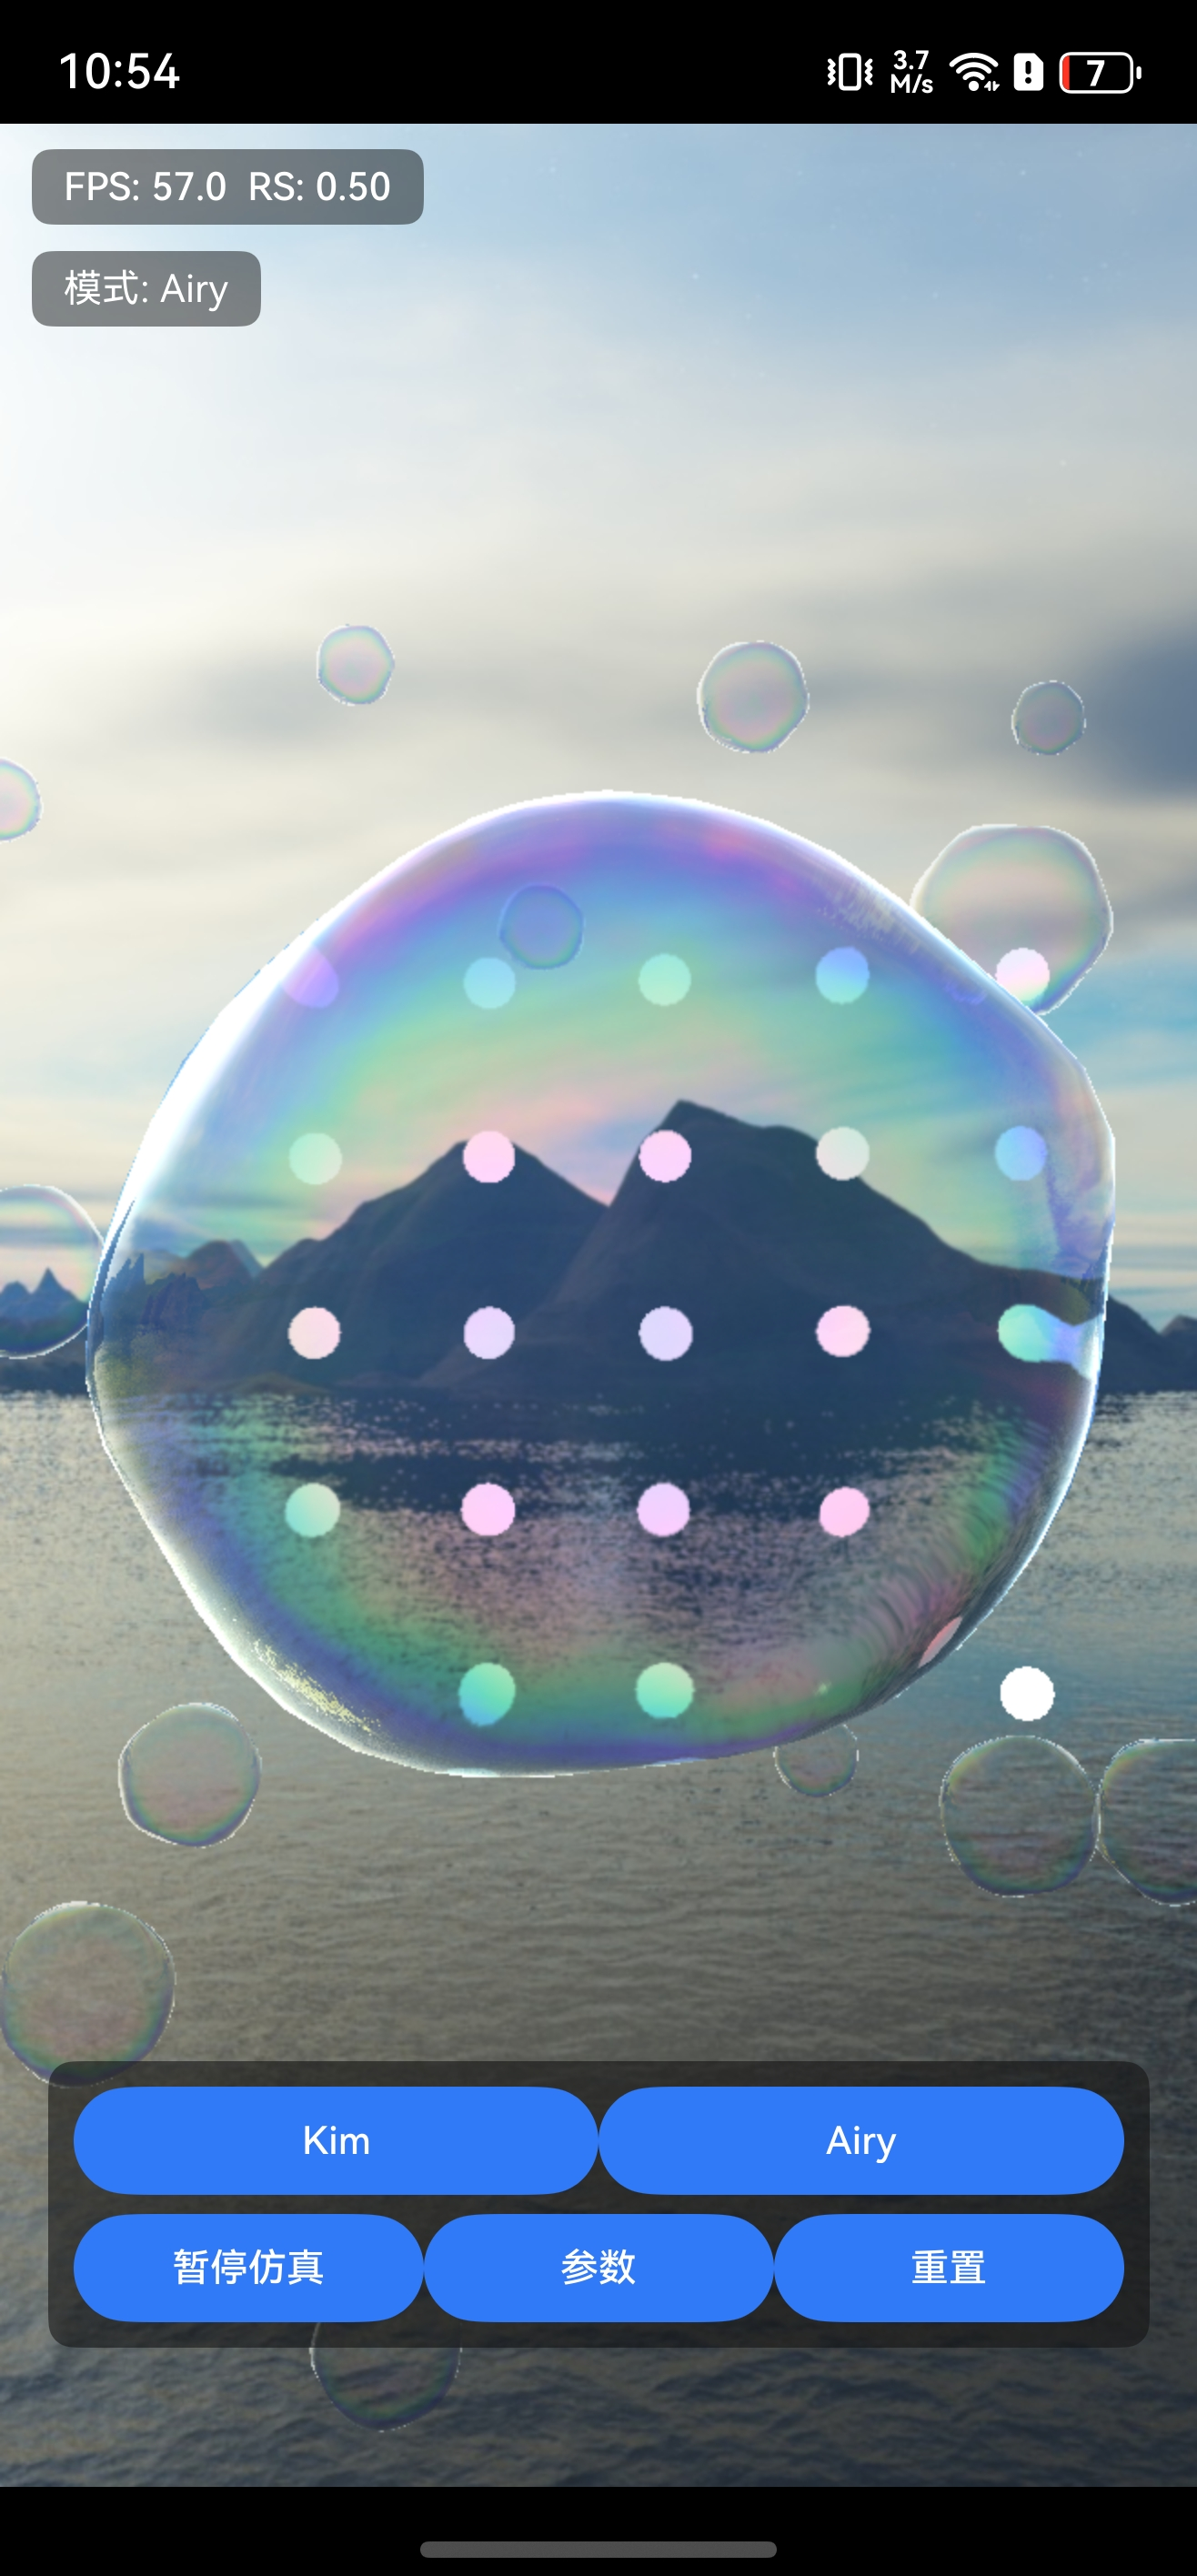
\includegraphics[height=5.65cm,trim=0 130 0 150,clip]{bubble_harm1.jpg}
      \par\vspace{0.1cm}
      \scriptsize\color{Gray}主泡泡折射与多泡泡场景
    \column{0.33\textwidth}
      \centering
      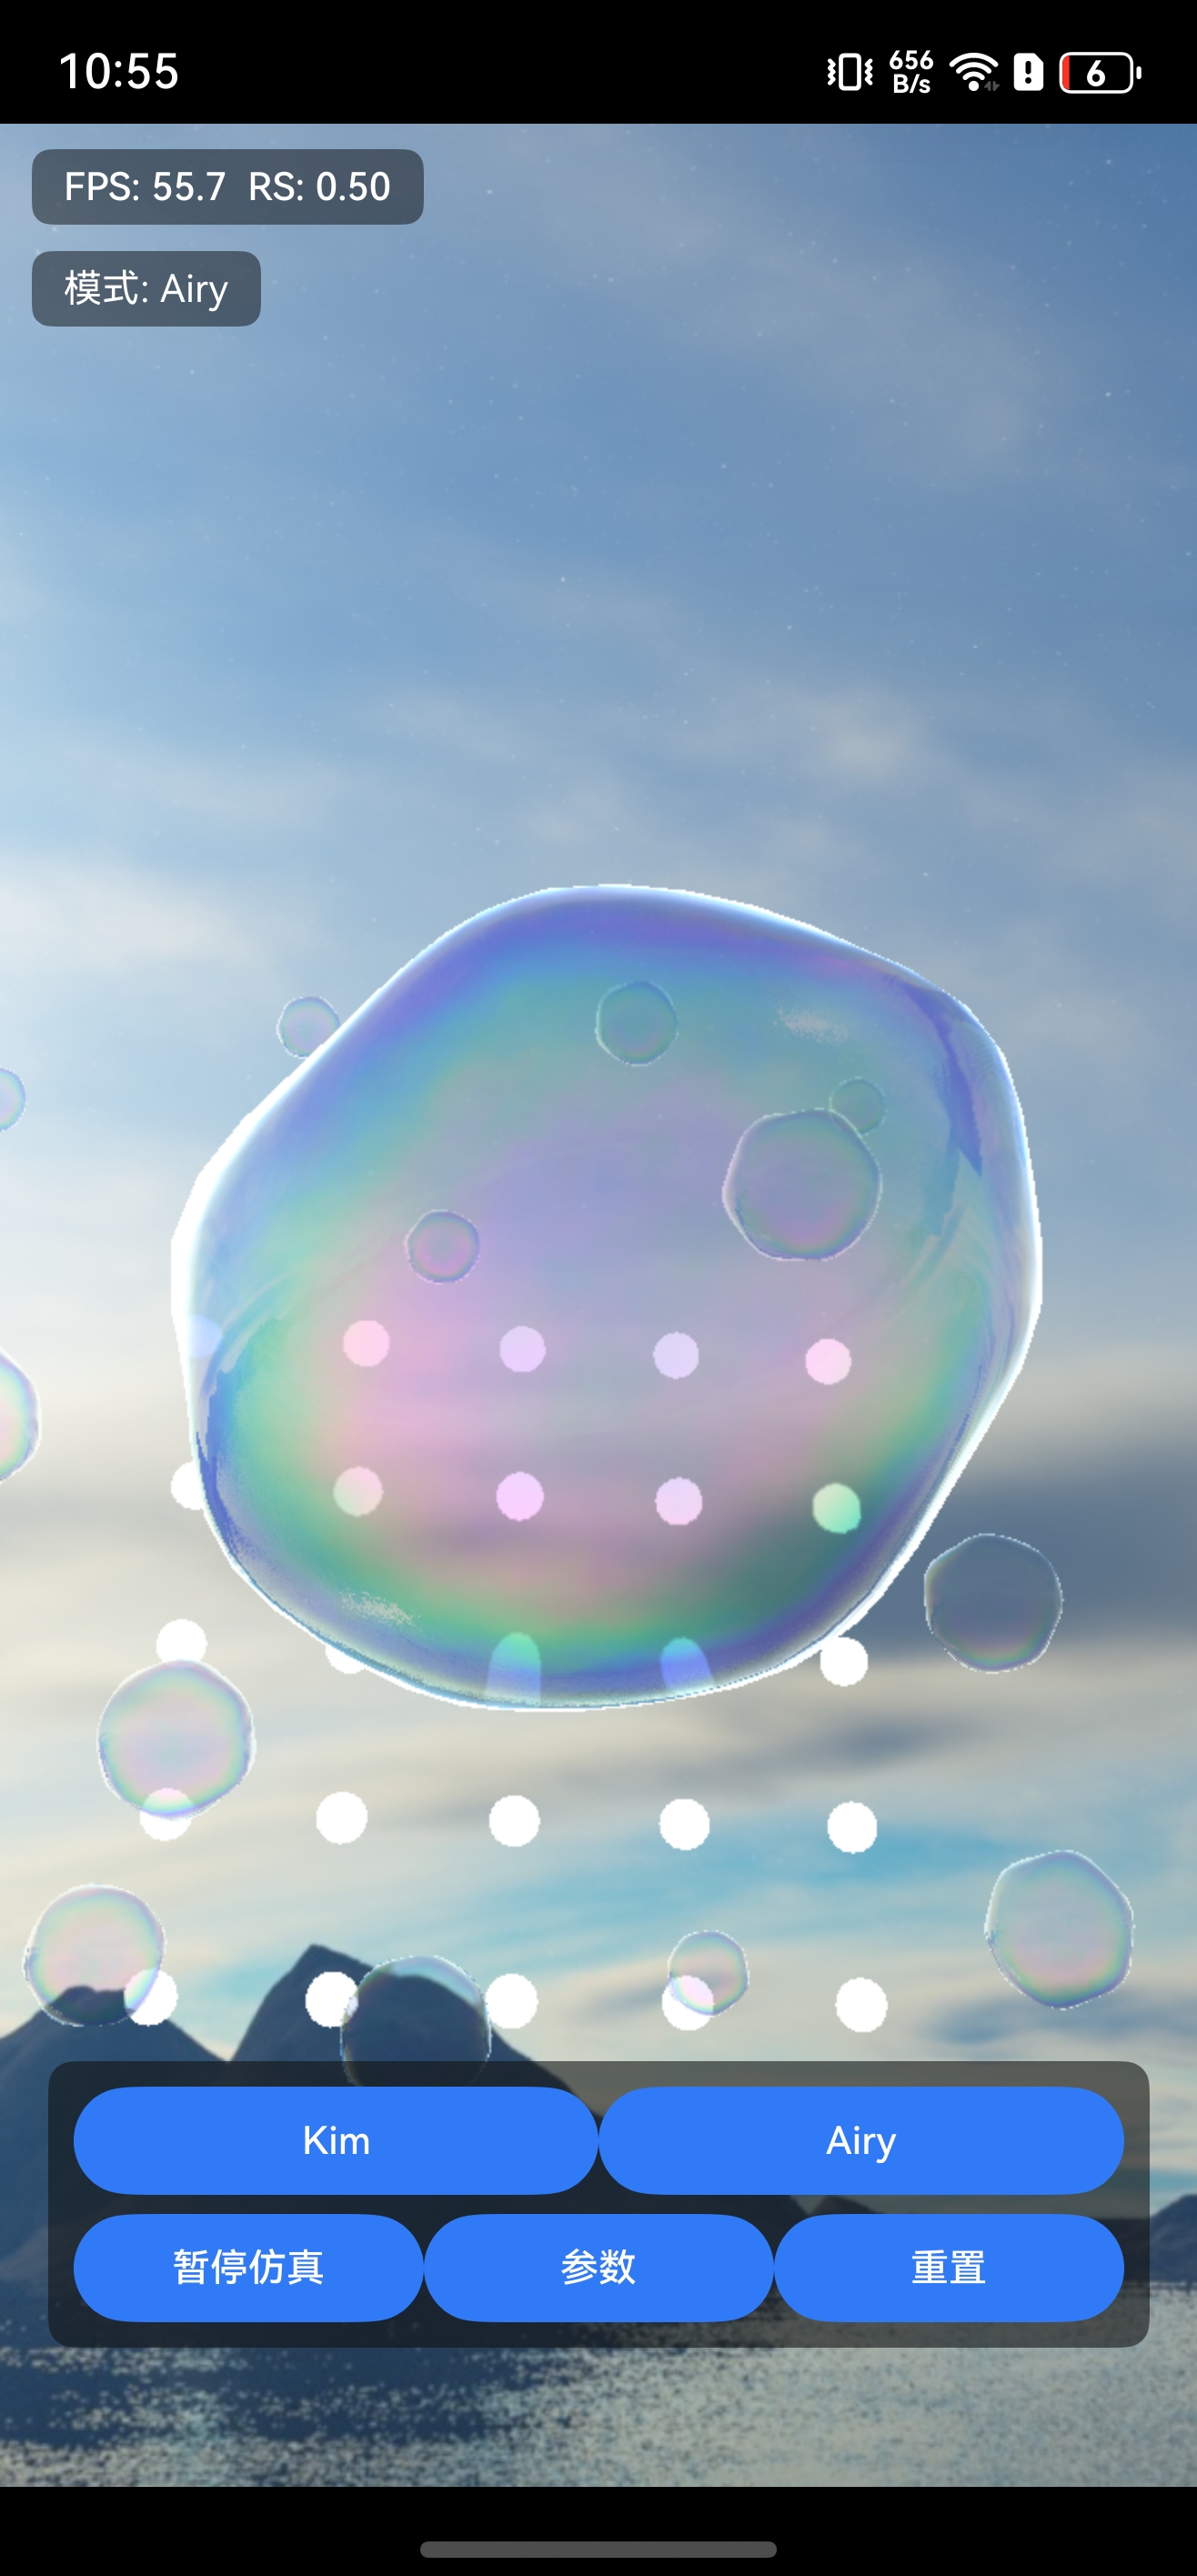
\includegraphics[height=5.65cm,trim=0 130 0 150,clip]{bubble_ham2.jpg}
      \par\vspace{0.1cm}
      \scriptsize\color{Gray}DBSTT 风格轮廓形变
    \column{0.30\textwidth}
      \textbf{截图记录}
      \begin{itemize}\setlength\itemsep{0.42em}
        \item HarmonyOS 真机
        \item OpenGL ES 3.0
        \item 默认 Airy 模式
        \item 内部渲染比例 0.50
        \item 截图 FPS：55.7 / 57.0
      \end{itemize}
      \vspace{0.25cm}
      {\scriptsize\color{Gray}
      结果表明系统已完成从 ArkTS 页面、NAPI、EGL 到 Native 渲染的端到端运行。}
  \end{columns}
\end{frame}

\begin{frame}{结果分析、局限与后续方向}
  \begin{columns}[T,onlytextwidth]
    \column{0.47\textwidth}
      {\color{Blue}\large\bfseries 已实现}\par
      \vspace{0.15cm}\color{Line}\rule{\linewidth}{.7pt}
      \begin{itemize}\setlength\itemsep{0.43em}
        \item 多阶段 FBO 双界面折射近似
        \item 两种薄膜虹彩与动态膜厚
        \item 触摸局部折射和色散响应
        \item 单泡泡 DBSTT 风格表面动态
        \item 多泡泡漂移、排序与 Alpha 合成
        \item HarmonyOS UI、Native 渲染与真机运行
      \end{itemize}
    \column{0.47\textwidth}
      {\color{Orange}\large\bfseries 局限与改进}\par
      \vspace{0.15cm}\color{Line}\rule{\linewidth}{.7pt}
      \begin{itemize}\setlength\itemsep{0.43em}
        \item 屏幕空间方法不能折射屏幕外对象
        \item Airy 为实时简化，尚非完整微表面预积分
        \item 膜厚变化未求解完整表面流体方程
        \item DBSTT 不支持泡沫拓扑变化与 Plateau 边界
        \item 展示泡泡尚无碰撞和流体耦合
        \item 后续补强相互折射、碰撞与更多真机性能数据
      \end{itemize}
  \end{columns}
\end{frame}

\begin{frame}{总结}
  \begin{columns}[T,onlytextwidth]
    \column{0.58\textwidth}
      \vspace{0.25cm}
      \begin{itemize}\setlength\itemsep{0.68em}
        \item 在 HarmonyOS 上实现了可运行、可交互的透明泡泡实时渲染系统
        \item 用多阶段 FBO 在移动端预算下近似双界面折射
        \item 将薄膜干涉、动态膜厚、环境反射和触摸响应统一到材质管线
        \item 以简化 DBSTT 与低成本漂移构建动态、多层次的泡泡场景
        \item 真机截图显示 Airy 模式下运行帧率约为 56--57 FPS
      \end{itemize}
      \vspace{0.4cm}
      {\color{Blue}\large\bfseries 光学模型、动态模拟与鸿蒙工程实现形成完整闭环。}
    \column{0.38\textwidth}
      \centering
      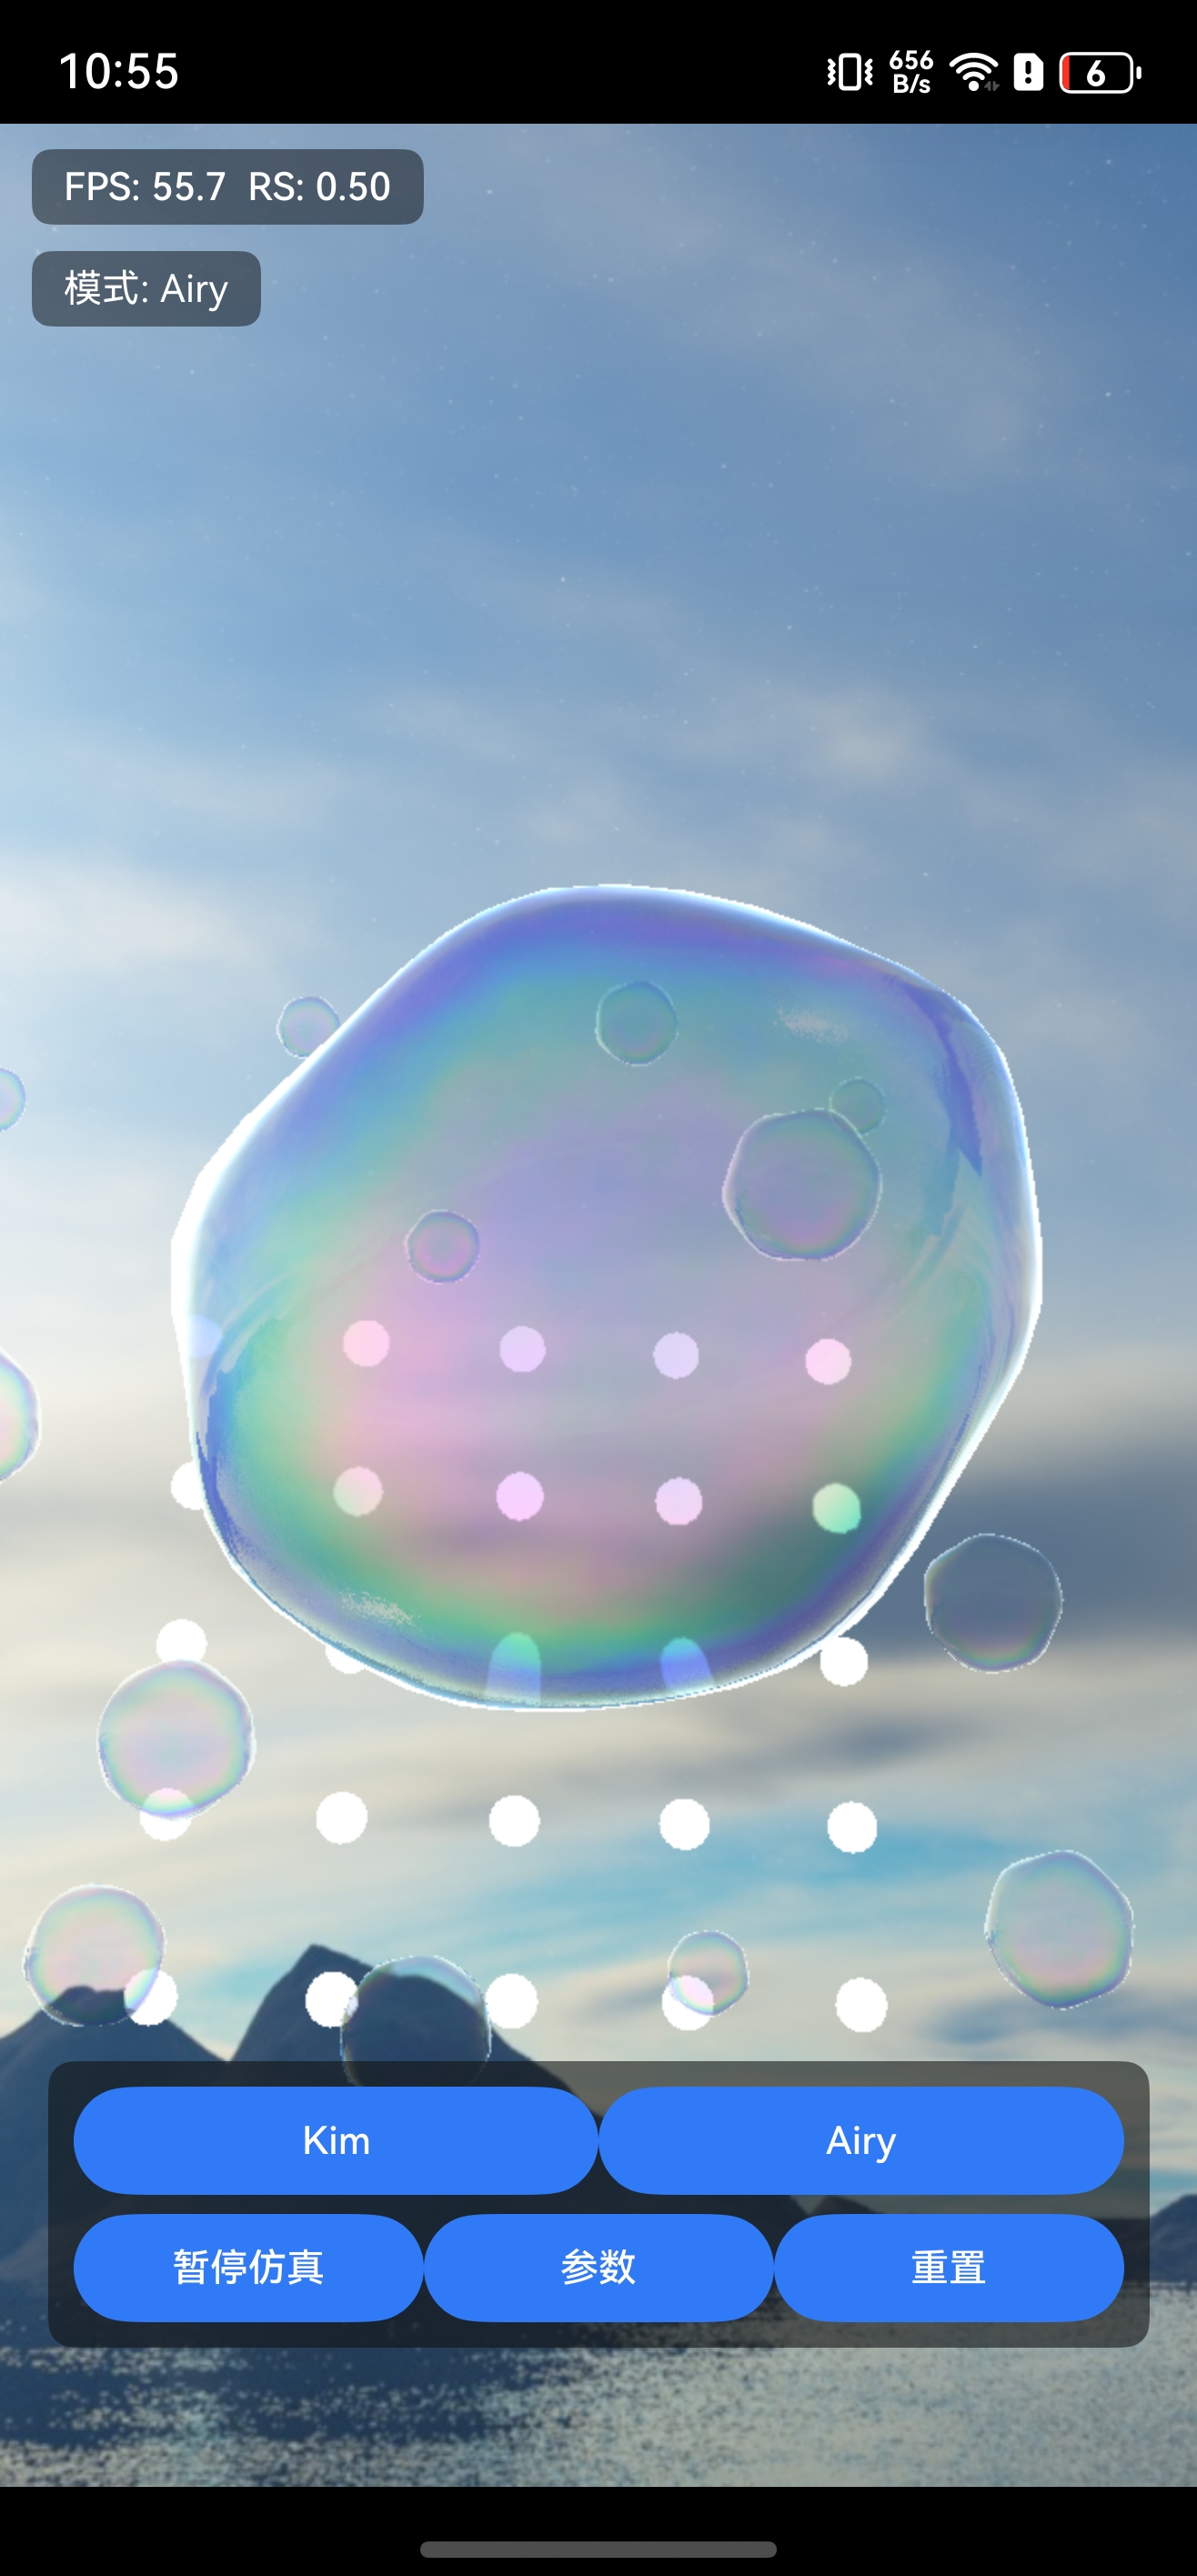
\includegraphics[height=6.0cm,trim=0 170 0 160,clip]{bubble_ham2.jpg}
  \end{columns}
\end{frame}

\begin{frame}{主要参考文献}
  \small
  \begin{enumerate}\setlength\itemsep{0.48em}
    \item Wyman C. \textit{An Approximate Image-Space Approach for Interactive Refraction}. SIGGRAPH Sketches, 2005.
    \item Kim N., Park K. \textit{Real Time Rendering Iridescent Colors Appearing on Soap Bubbles}. Springer, 2012.
    \item Iwasaki K., Matsuzawa K., Nishita T. \textit{Real-Time Rendering of Soap Bubbles Taking into Account Light Interference}. CGI, 2004.
    \item Belcour L., Barla P. \textit{A Practical Extension to Microfacet Theory for the Modeling of Varying Iridescence}. ACM TOG, 2017.
    \item Ishida S. et al. \textit{A Model for Soap Film Dynamics with Evolving Thickness}. ACM TOG, 2020.
    \item Da F. et al. \textit{Double Bubbles Sans Toil and Trouble: Discrete Circulation-Preserving Vortex Sheets for Soap Films and Foams}. ACM TOG, 2015.
  \end{enumerate}
\end{frame}

{\setbeamertemplate{footline}{}
\begin{frame}[plain]
  \vfill
  \begin{center}
    \begin{minipage}{0.55\textwidth}
      \centering
      {\color{Cyan}\rule{1.05cm}{2pt}}\par
      \vspace{0.55cm}
      {\fontsize{28}{34}\selectfont\bfseries\color{Navy}谢谢！}\par
      \vspace{0.35cm}
      {\large\color{Blue}Q \& A}\par
      \vspace{0.8cm}
      {\small\color{Gray}
      队伍：吃福是亏\\
      杨弘宇、常毅寒、杨硕、高凡、赵艺博}
    \end{minipage}
  \end{center}
  \vfill
\end{frame}}

\end{document}
